\clearpage\nobalance
\section*{Author Notes}
\subsection*{Full Acknowledgments}
Yiqiao Liu thanks Professor Luyao Zhang for the COMSCI/ECON 206 assignment, official templates, and emphasis on evidence-linked interdisciplinary research; Professor Kenneth S. (Ken) Rogerson for his documented role in the course's 7 September 2026 “2056 Nobel and Turing Laureate Program Launch Workshop” context (no direct FP10 paper review is claimed); Han Zhang for the author-supplied suggestion to study an independent third-party oversight extension; and Xinrong Sun for the author-supplied novelty, domain-necessity, congestion-benefit, and CCAR-externality challenges. Exact dates/wording of the latter two records await author confirmation. We acknowledge Tencent's Shanghai office, the Shanghai Science and Technology Museum, and the COMSCI/ECON 206 classroom community as course field-learning/community contexts, without attributing unrecorded FP10 findings to them. Official UN SDG assets are credited to the United Nations. Python, NumPy, Matplotlib, nbclient, Gradio, Chromium/Playwright, the ACM class, and the instructor-supplied templates supported the artifacts. OpenAI Codex assisted the final audit, code verification, drafting, figures, and production; Yiqiao Liu remains responsible for every claim, source, computation, and submission.

\subsection*{Updated Team and Individual Contributions}
\textbf{Team FP10 is a solo project.} Yiqiao Liu chose to preserve a three-action Bayesian disclosure game, distinguish mandatory safety information from voluntary commercial detail, interpret full information as an infeasible reference, and test CCAR as a candidate rather than an optimum. Liu authored and verified \texttt{src/}, \texttt{tests/}, the two notebooks, the Hugging Face/static demo, deterministic result manifests, paper, diagrams, and poster. Verification includes exhaustive 81-profile equilibrium enumeration, welfare arithmetic, 760-cell robustness, belief/tolerance sensitivities, local notebook execution, automated tests, and rendered artifact inspection. The integrated consequence is that computation found failure regions, which narrowed both the mechanism and practical-impact claims and shaped the behavioral/institutional roadmap.

\bibliographystyle{ACM-Reference-Format}\bibliography{references}

\appendix
\section{Technical Details and Reproducibility}
\label{app:technical}
For type-contingent strategies $s_i$, interim expected utility is
\[EU_i(a\mid t_i,s_j,d)=\sum_{t_j}\Pr(t_j)u_i(a,s_j(t_j);t_i,d).\]
A profile is a pure BNE iff each prescribed action maximizes this expression for both types and both players. The implementation enumerates all $3^2$ strategies per player and all 81 pairs, preserving all ties within tolerance $10^{-10}$. For each realized type pair the first best enumerates nine action profiles, maximizes $u_A+u_B$, preserves ties, and averages under the prior. The gap is exactly $W_{FB}-W_{BNE}$, evaluated using underlying welfare even when CCAR modifies access utility.

\begin{table}[H]\centering\small\caption{Verified normalized primitives and benchmark.}
\begin{tabular}{@{}lllll@{}}\toprule
State & BNE $(L,H)$ & $W_{BNE}$ & $W_{FB}$ & Gap\\\midrule
Low $(d=.3)$ & $(M,M)$ & 0.000 & 0.639 & 0.639\\
Medium $(d=.6)$ & $(P,M)$ & 2.193 & 3.139 & 0.946\\
High $(d=1)$ & $(P,P)$ & 6.882 & 7.385 & 0.503\\\bottomrule
\end{tabular}\end{table}

CCAR input is congestion, own disclosure action, and $\alpha_M$. Its output is an enhanced-information access factor: 1 at Low; $\alpha_M$ for Minimum at Medium/High; 1 for Partial/Full. It assumes observable/verifiable action, contains no report-quality model, has no administration/enforcement cost, and does not establish voluntary participation or incentive compatibility. At Medium and $\alpha_M=.7$, BNE is $(P,P)$ and underlying welfare is 3.089. The robustness grid is $2\times20\times19=760$ deterministic cells over Medium/High, $c_H=1.1,\ldots,3.0$, and $\alpha_M=.1,\ldots,1.0$. Categories overlap.

Reproduction: create the specified Python environment, run \texttt{python scripts/build\_final\_evidence.py}, then the four test commands in the README. No random seed enters the equilibrium results. The allocation simulation uses seed 206. Environment captured during evidence generation: Python 3.13.7, NumPy 2.3.5, Matplotlib 3.10.8. Known limits: two symmetric operators; independent binary types; three discrete actions; exogenous congestion; pure strategies; uncalibrated normalized primitives; no report accuracy, implementation cost, mixed equilibrium, dynamics, or empirical sample. The exact final tested commit is intentionally inserted only after final commit and rerun.

\subsection{AI Use Disclosure}
OpenAI Codex (GPT-5-family coding agent; exact backend build not exposed) was used on 15 October 2026 for repository/requirements audit, computation and test verification, source checking, academic editing, diagrams, paper/poster production, and release validation. The material prompt is the author's final-project master instruction retained in the Codex task record. Accepted work includes the central evidence builder, bounded literature comparison, failure-case reporting, release documents, and layout drafts. Rejected/qualified suggestions include absolute novelty, universal welfare improvement, empirical aviation or behavior claims, fabricated human activity, and successful deployment without evidence. Automated checks are logged in the release documentation. Human scientific, visual, historical-credit, and submission review remains pending; Yiqiao Liu bears responsibility.

\section{Cumulative Intellectual Development}
Verified continuity begins with the tracked PS2 drone-disclosure repository at commit \texttt{6baa4107}. The final revision preserves its player/type/action space, welfare benchmark, CCAR, allocation exercise, notebooks, and decision lab. The 15 October audit added a central evidence source, belief/tolerance sensitivities, explicit category overlap, three closest-paper verification, and diagrams. Han Zhang's supplied three-party suggestion became a roadmap test rather than a claimed feature. Xinrong Sun's supplied objections caused four consequential revisions: narrow novelty; label drone claims as application interpretation; expose congestion benefit as an assumption; and foreground CCAR no-effect/adverse regions. Week 1, Week 2, PS1, October 12, October 14, workshop, Ed, email, and handwritten records are not present in the repository; their detailed historical content remains pending rather than inferred.

\section{Open Source and Three Lens Inspiration}
Game theory supplies Bayesian strategies and best-response conditions; social choice distinguishes individual utility from aggregate welfare and exposes omitted distributional criteria; mechanism design changes enhanced-access payoffs and tests implementation trade-offs. Python/NumPy implement exhaustive deterministic enumeration; Matplotlib produces reproducible figures; nbclient supports clean local notebook execution; Gradio/static HTML provide an illustrative decision interface. Official UN icons remain UN property and are used for academic communication with source attribution. The ACM/instructor LaTeX and A0 templates define delivery structure. The repository's own license governs project reuse; third-party components retain their licenses.

\section{Feedback Response and Revision Record}
\begin{table}[H]\small\centering\caption{Consequential feedback responses.}
\begin{tabularx}{\columnwidth}{@{}p{1.5cm}p{2.1cm}YY@{}}\toprule Source & Challenge & Decision and revision & Verification / open issue\\\midrule
Han Zhang & Three-party oversight & INVESTIGATE: roadmap adds independent coordinator & Current solver remains two-player; original record needed\\
Xinrong Sun & Los et al. novelty & REVISE: exact three-paper comparison; bounded contribution & DOI/publisher metadata checked; intended citation needs confirmation\\
Xinrong Sun & Drone necessity / congestion assumption & REVISE: abstraction boundary and sensitivity & Code/model and grid inspected; no calibration\\
Xinrong Sun & CCAR externalities & REVISE: report no-effect, excessive, larger-gap, multiplicity & 760 cells recomputed\\
Official assignment & Final artifacts and structure & REVISE: official paper/poster template and release checks & Build record in Appendix G\\\bottomrule
\end{tabularx}\end{table}
The repository's final-documentation folder contains the complete machine-readable feedback register. Direct FP10 feedback from Ken Rogerson is not claimed.

\clearpage\onecolumn
\section{Structured Abstract and Cumulative Proposal Map}
\begin{table}[H]\caption{Eight required parts and consequential final revision.}\renewcommand{\arraystretch}{1.12}
\begin{tabularx}{\textwidth}{@{}p{0.18\textwidth}Y@{}}\toprule Part & Current statement and revision evidence\\\midrule
Background & Competing operators choose non-safety disclosure under private confidentiality cost and public congestion; three closest papers verified.\\
Motivation & Private incentives can miss aggregate welfare, but more disclosure is not always better.\\
Application Scenario & Stylized low-altitude coordination; mandatory safety, emergencies, and empirical operations excluded.\\
Research Question & Conditions for equilibrium disclosure, welfare gaps, and CCAR improvement/failure.\\
Method & Complete Bayesian strategies, exhaustive pure-BNE enumeration, first best, deterministic robustness.\\
Results & Benchmark reproduced; Medium gap $0.946\rightarrow0.050$ under the example; adverse/no-effect regions reported.\\
Intellectual Merits & Bounded new model/application combination and comparative computation, not a theorem.\\
Practical Impacts & Prospective SDG 9.1/11.2 connection with indicators, risks, safeguards, and evidence labels.\\\bottomrule
\end{tabularx}\end{table}

\section{Retained PS2 Auction Artifact and Symposium Record}
The upstream disclosure game is not an auction. The downstream exercise allocates one residual commercial priority slot; emergency/public-safety missions are excluded from payment-based access. Participants have private scalar values and submit sealed bids. FCFS allocates to the first eligible request, charges zero, and stops. The alternative single-unit second-price auction allocates to the highest bid, charges the second-highest bid, breaks ties by operator ID, and stops. Under the independent-private-values benchmark, truthful bidding is weakly dominant \cite{vickrey1961counterspeculation}. For values $(8,5,3,2)$ and arrival B,C,A,D, FCFS chooses B (efficiency .625); second price chooses A, payment 5, utility 3 (efficiency 1). In 10,000 seed-206 draws, mean FCFS efficiency is .622308, second-price efficiency 1, and auction revenue 5.99207. This illustrates scarcity allocation only; it does not establish aviation legitimacy, distributional fairness, willingness/ability-to-pay equivalence, or CCAR performance. A documented 28 September symposium record was not recovered and awaits the author.

\section{Final Week Evidence and Final Release Audit}
\textbf{Evidence status.} October 12 Ed post, duet thread, Category I/II/III posts, and October 14 peer replies, roundtable, Ken Rogerson exchange, and handwritten exit records were not recovered. They remain structured placeholders in \texttt{docs/final/final\_week\_evidence.md}. Known Han Zhang/Xinrong Sun summaries are used only as author-supplied summaries. No fictional transcript, date, or participant is supplied.

\begin{figure}[H]\centering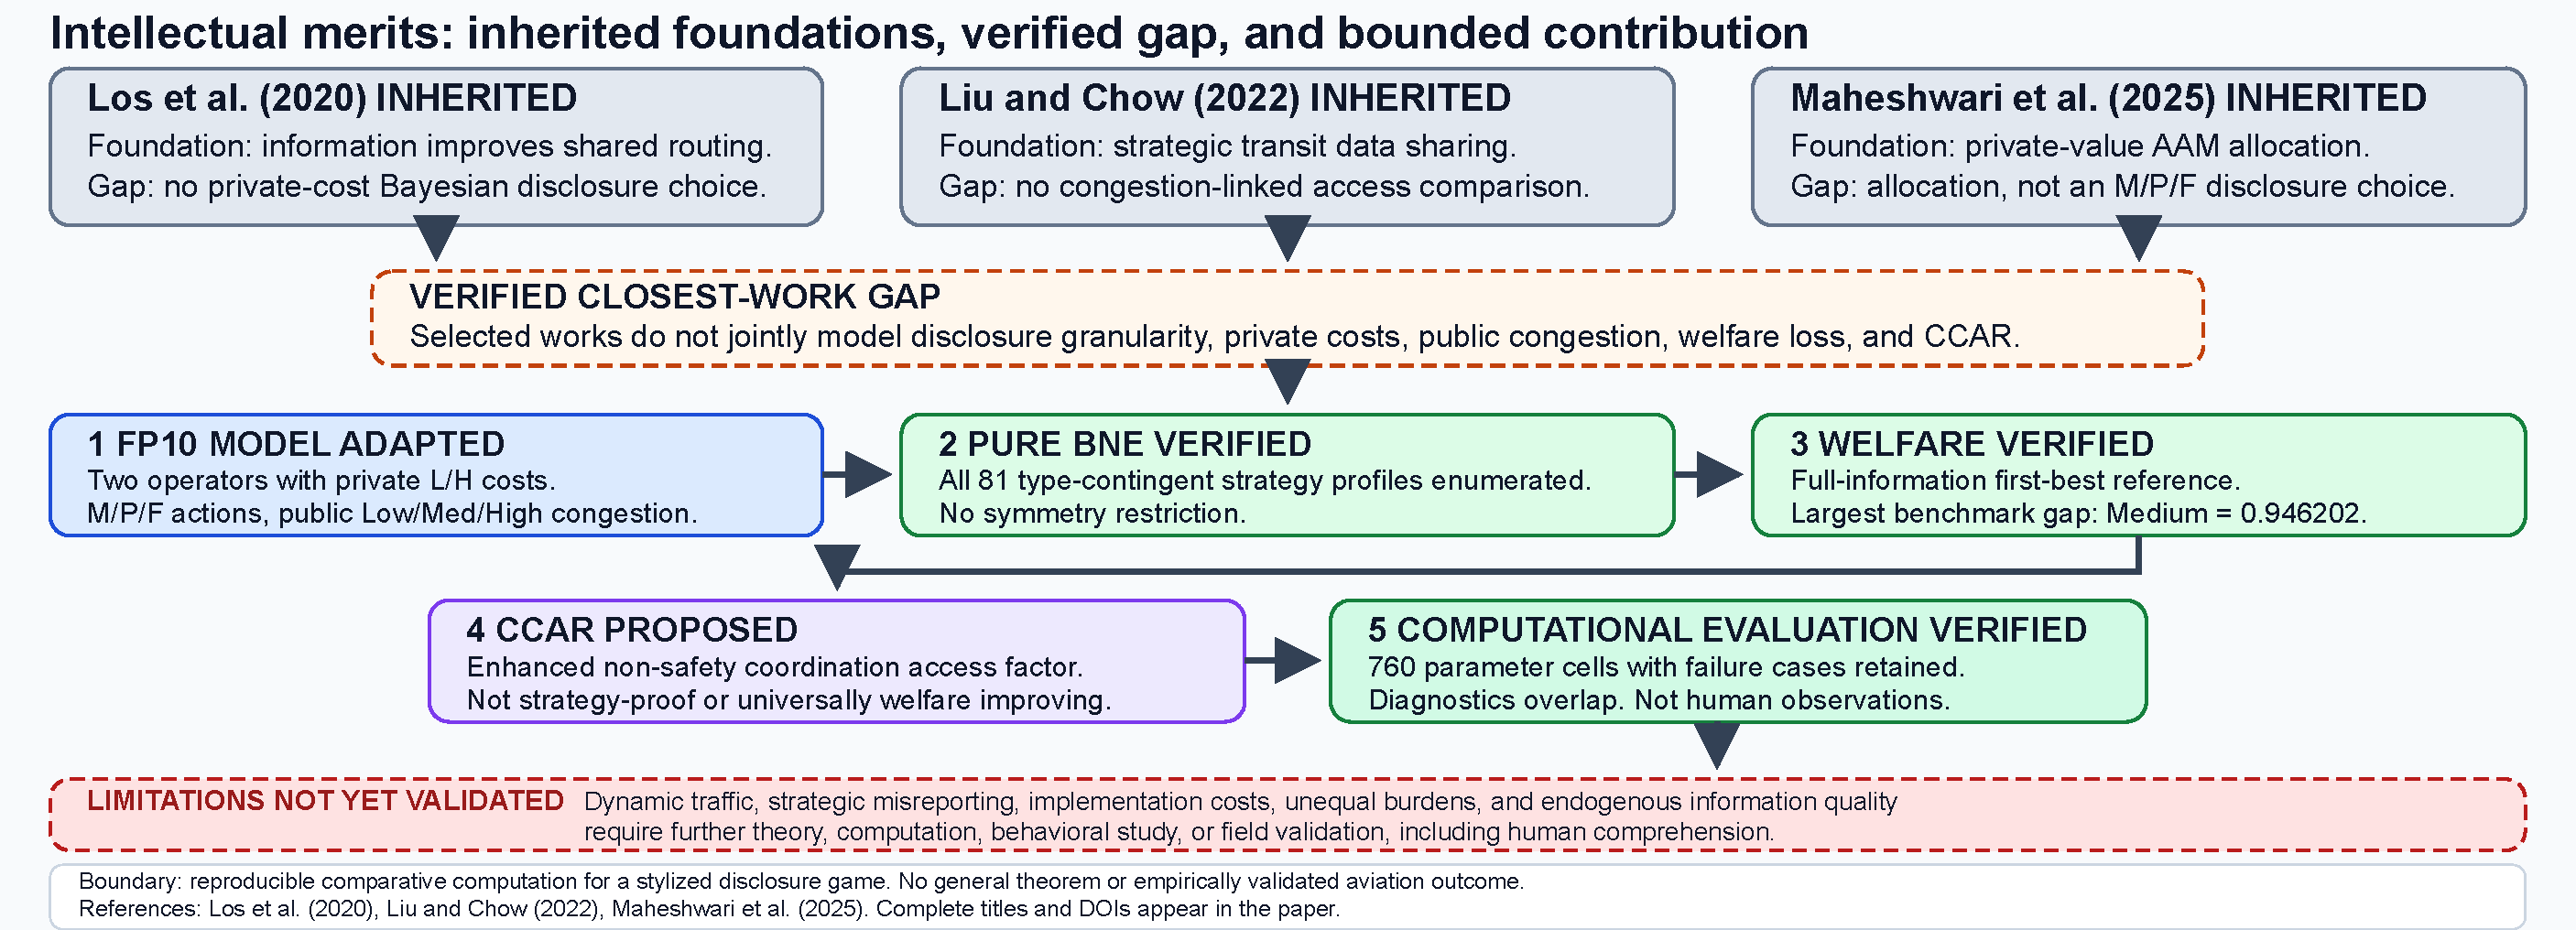
\includegraphics[width=.96\textwidth]{figures/intellectual_merits.pdf}\caption{Expanded Intellectual Merits chain. Blue denotes inherited literature; teal denotes project computation; yellow denotes limitations/proposed tests.}\end{figure}
\begin{figure}[H]\centering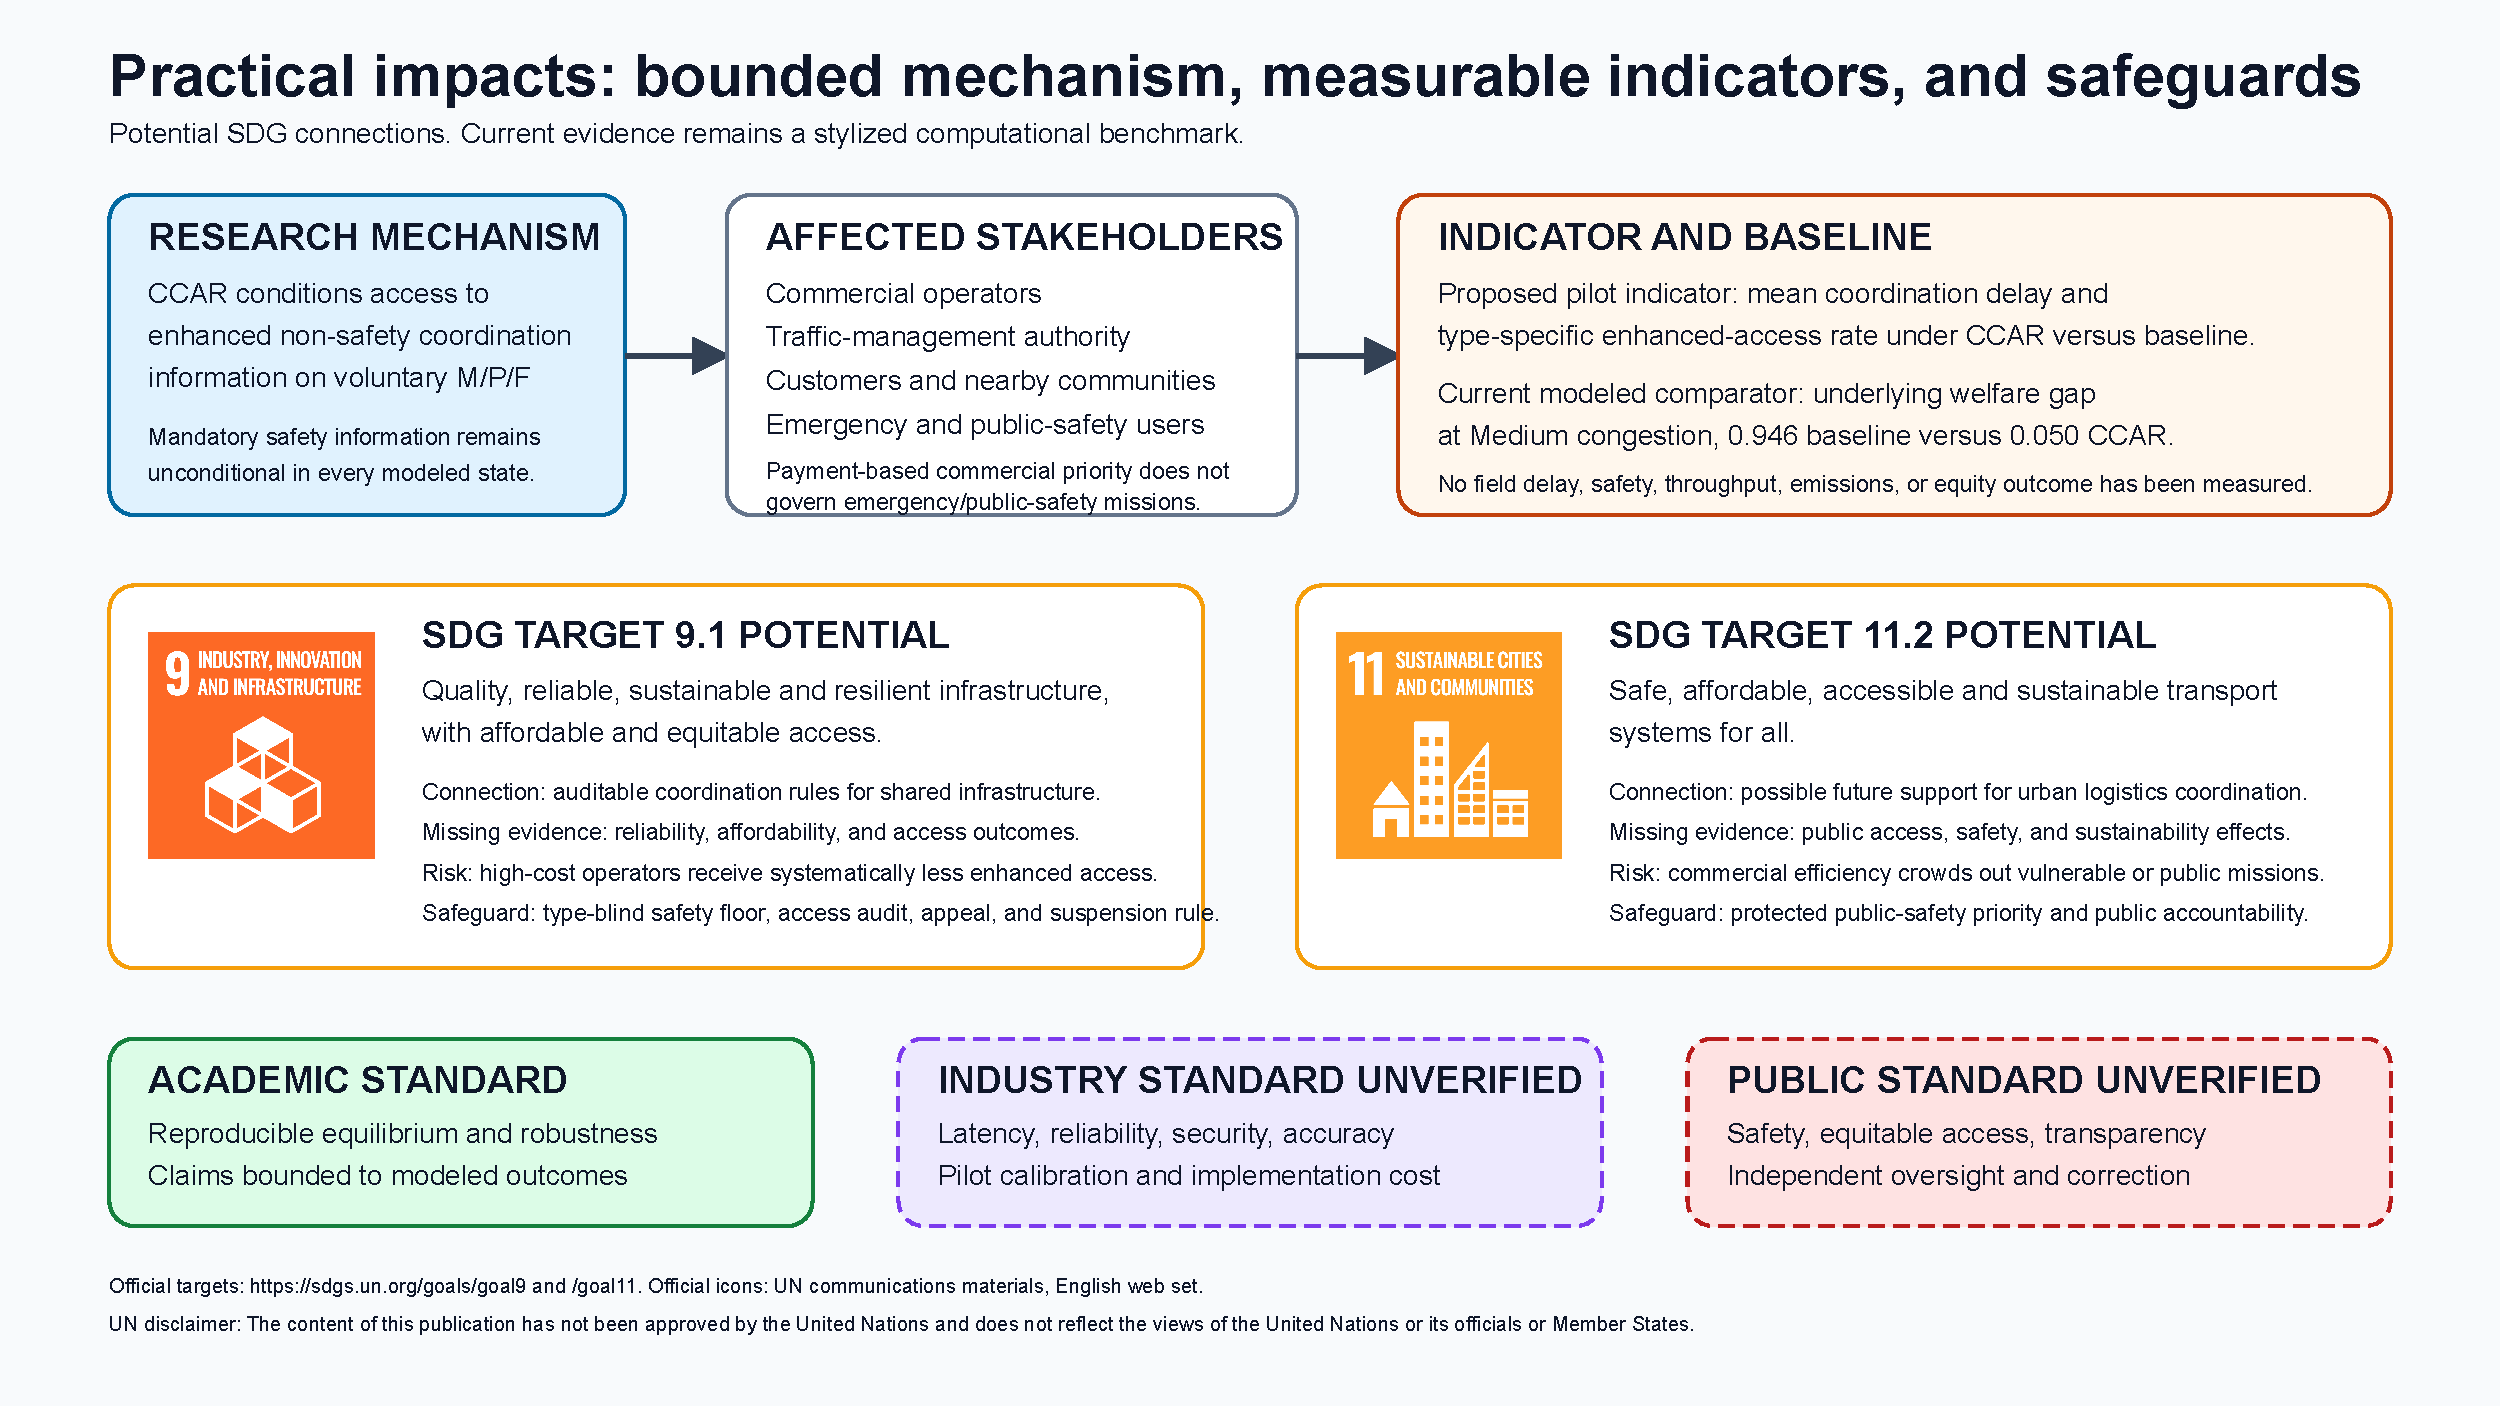
\includegraphics[width=.96\textwidth]{figures/practical_impacts.pdf}\caption{Prospective impact map using official UN Goal 9 and 11 icons. Only stylized computational evidence is demonstrated.}\end{figure}
\begin{figure}[H]\centering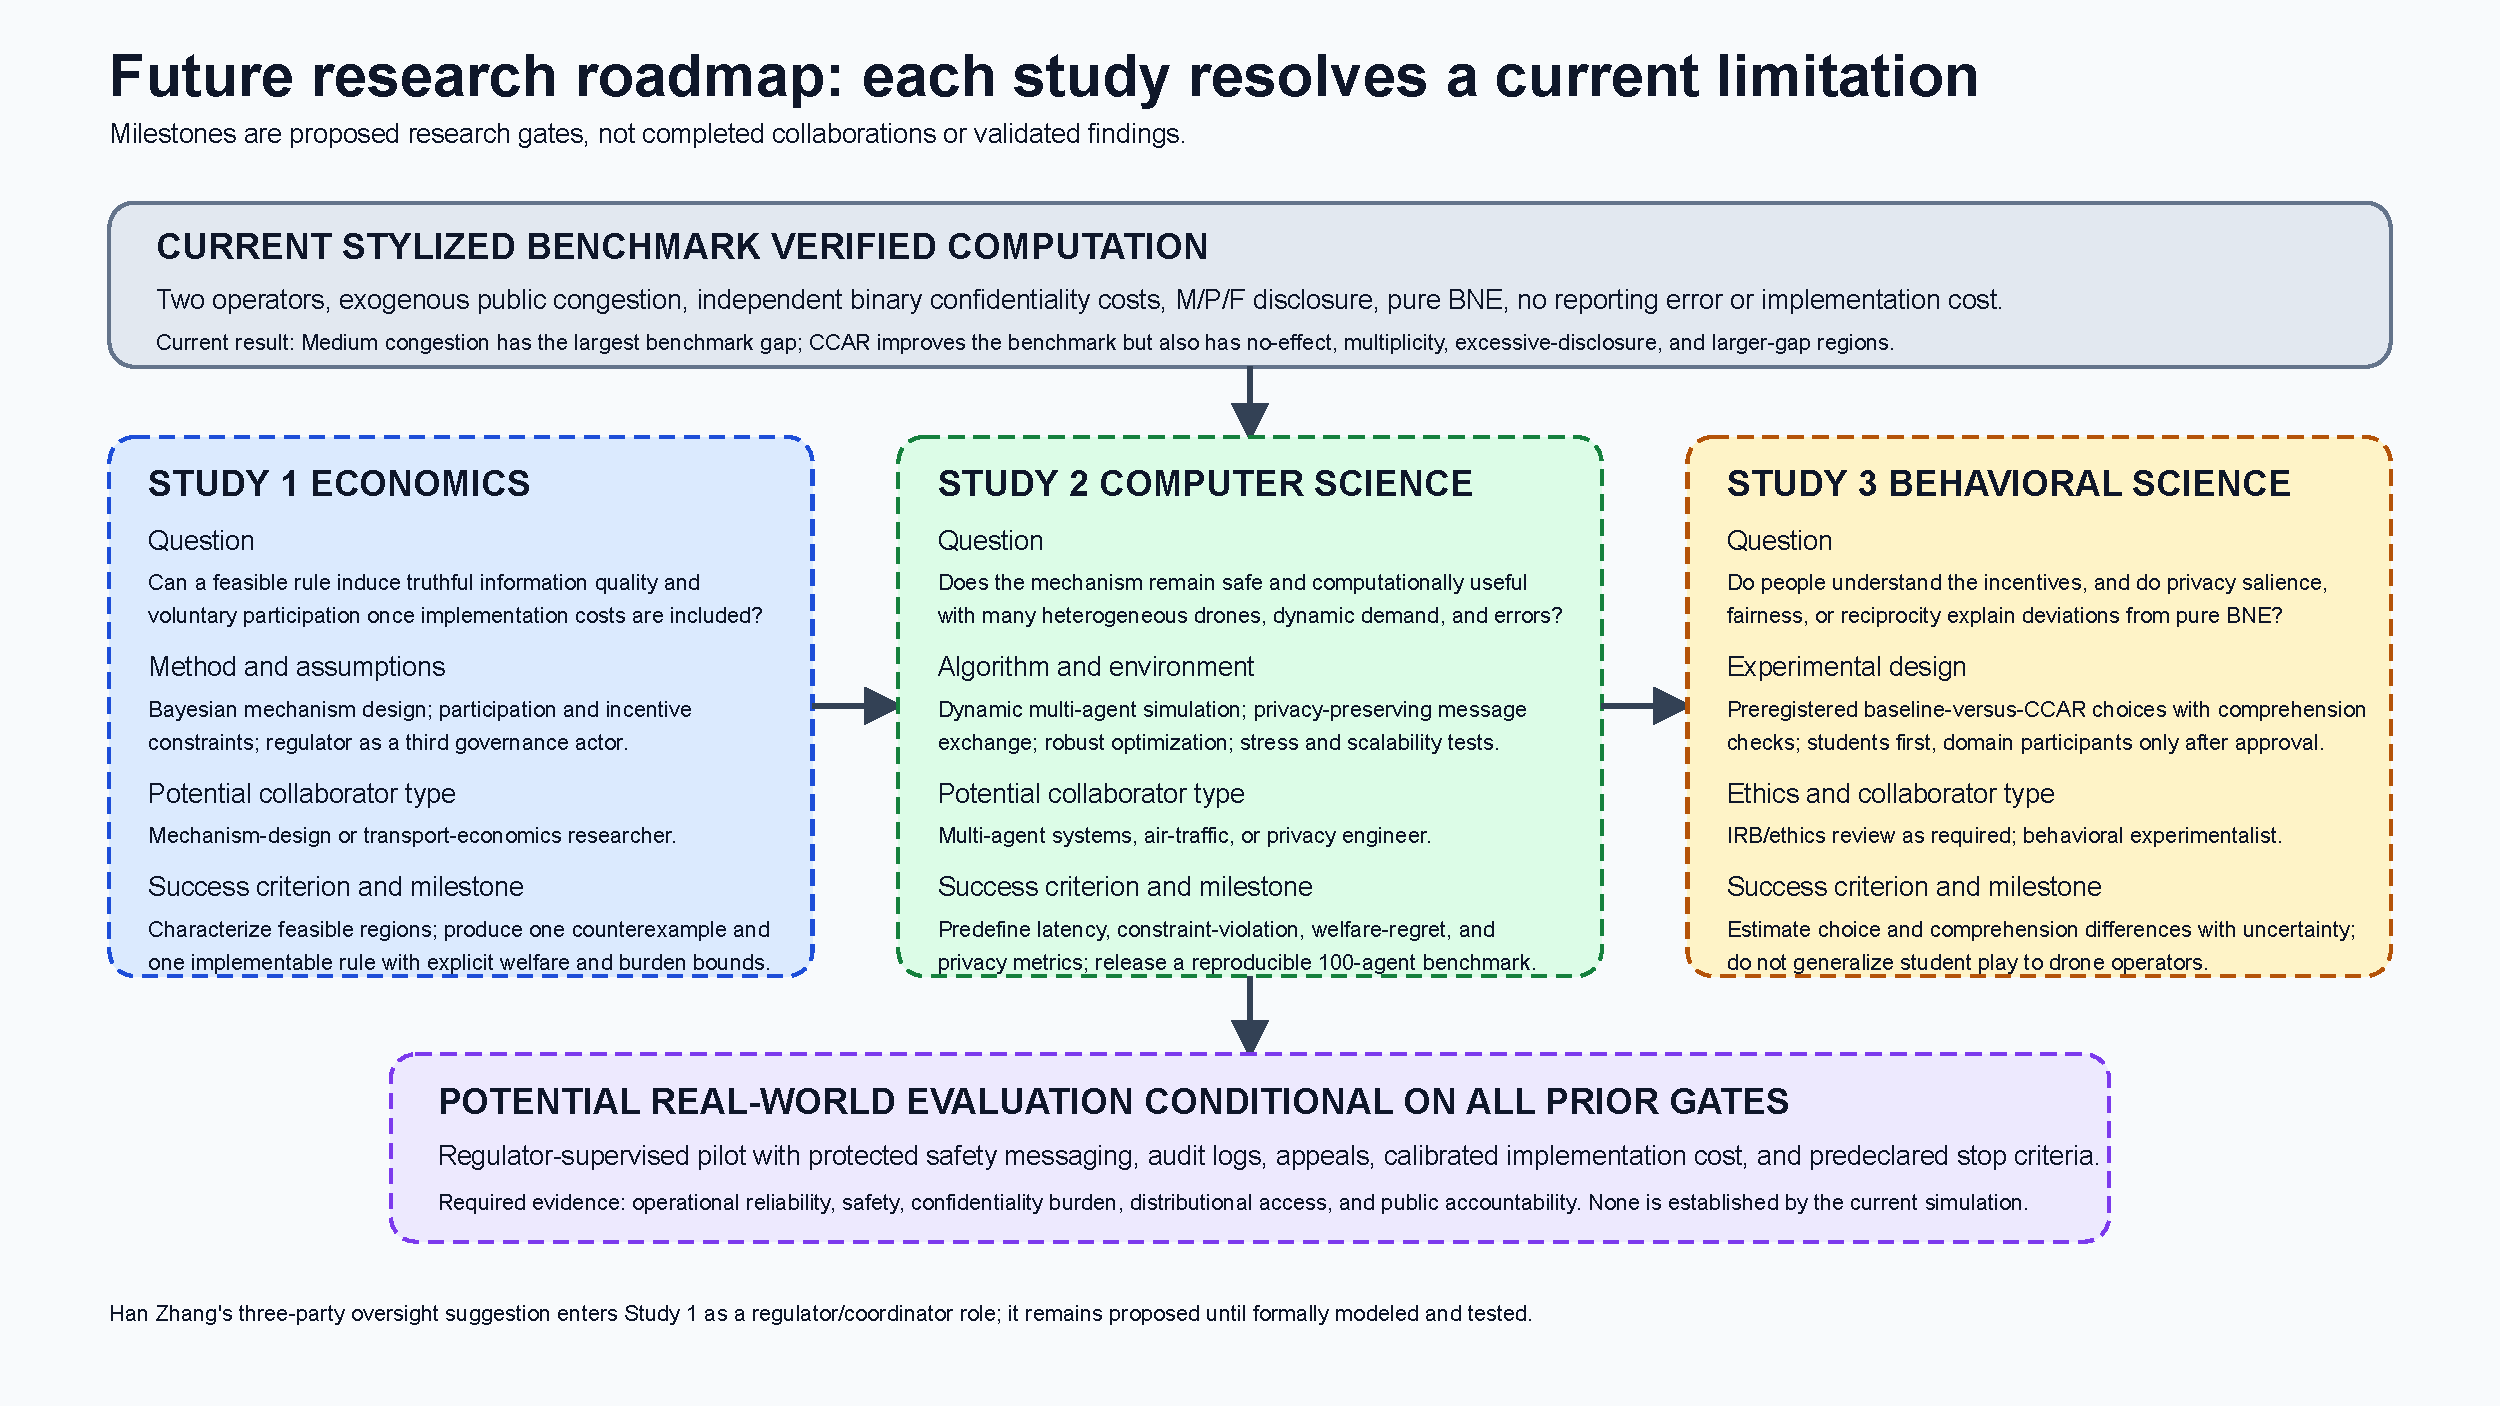
\includegraphics[width=.96\textwidth]{figures/research_roadmap.pdf}\caption{Future roadmap linking current limitations to economics, computer-science, behavioral, and institutional tests.}\end{figure}

\textbf{Nobel comparison.} Official records identify the 2025 prize to Joel Mokyr, Philippe Aghion, and Peter Howitt for innovation-driven growth, and the 2026 prize jointly to Robert E. Hall and Michael Woodford for microeconomic foundations of macroeconomic stabilisation. The comparison motivates linking agent-level incentives to long-run institutional outcomes; it does not validate FP10 or imply prize merit.

\textbf{Release audit.} The root README embeds \texttt{poster/final-poster.png} and links \texttt{poster/final-poster.pdf}. Final package paths, hashes, tests, notebook records, paper main-page count, PPTX slide geometry, PDF inspection, acknowledgments, AI disclosure, and unresolved manual checks are recorded in \texttt{docs/final/release\_readiness.md} and \texttt{outputs/final/release\_manifest.json}. Final author confirmation is pending.
